% interactnlmsample.tex
% v1.05 - August 2017

\documentclass[]{interact}

\usepackage{epstopdf}% To incorporate .eps illustrations using PDFLaTeX, etc.
\usepackage[caption=false]{subfig}% Support for small, `sub' figures and tables
%\usepackage[nolists,tablesfirst]{endfloat}% To `separate' figures and tables from text if required
%\usepackage[doublespacing]{setspace}% To produce a `double spaced' document if required
%\setlength\parindent{24pt}% To increase paragraph indentation when line spacing is doubled

\usepackage[numbers,sort&compress]{natbib}% Citation support using natbib.sty
\bibpunct[, ]{[}{]}{,}{n}{,}{,}% Citation support using natbib.sty
\renewcommand\bibfont{\fontsize{10}{12}\selectfont}% Bibliography support using natbib.sty
\makeatletter% @ becomes a letter
\def\NAT@def@citea{\def\@citea{\NAT@separator}}% Suppress spaces between citations using natbib.sty
\makeatother% @ becomes a symbol again


\begin{document}

\articletype{}% Specify the article type or omit as appropriate

\title{Indicators for effects on mean and variance in projected normal regression models for a circular outcome}

\author{
\name{Jolien Cremers\textsuperscript{a}\thanks{Corresponding author: J. Cremers, email: joliencremers@gmail.com} and Daniel Hernandez-Stumpfhauser\textsuperscript{b}}
\affil{\textsuperscript{a}Department of Methodology and Statistics, Utrecht University ; \textsuperscript{b}SAS Institute Inc., Cary, NC 27513, USA}
}

\maketitle

\begin{abstract}
  Projected normal models for circular data are so called heterogeneous error
  models, the structure of the model allows for the simultaneous modelling of
  effects on the mean (a location effect) and variance (an accuracy effect) of a
  circular variable. In this paper we investigate several measures for assessing
  whether there is either just an effect on the variance or both an effect on
  the variance and the mean of the circular outcome in a circular regression
  model. In previous literature a measure to do so, the signed shortest distance
  to the origin ($SSDO$), has already been introduced. However, our simulations suggest
  that the type I error of the $SSDO$ is greater than the specified $\alpha$
  level. We introduce a hypothesis test based on an angle based measure that
  achieves, in our simulations, the correct type I error.
\end{abstract}

\begin{keywords}
circular regression; projected normal models; heterogeneous error
\end{keywords}


\section{Introduction}

Circular regression models are those in which a circular variable $\theta \in
[0, 2\pi)$ is regressed on a set of linear and/or circular predictors,
$\boldsymbol{x}$. In the literature there are three approaches to circular data,
the `intrinsic', `wrapping' and `embedding' approach \cite{mardia2000directional}.
In the intrinsic approach models are based on distributions directly defined on
the circle whereas in the wrapping and embedding approach distributions are
defined in respectively $\mathbb{R}$ and $\mathbb{R}^2$ and subsequently wrapped
or projected onto the circle. Within each of these three approaches regression
models for a circular outcome have been introduced \cite{fisher1992regression,
lagona2016regression, presnell1998projected, mulder2017bayesian,
ravindran2011bayesian, nunez2011bayesian}.

Another distinction that can be made in the literature on circular regression
models is one between models with homogeneous errors and those with
heterogeneous errors \cite{rivest2015general}. In a homogeneous error model predictor
variables can only affect the mean of the circular outcome while in heterogeneous
error models predictor variables can have an effect on both the mean  (a
location effect) and variance (an accuracy effect) of the circular outcome. The
projected normal (PN) regression model, the model we focus on in this paper, is
one of these heterogeneous error models for circular variables. This model was
first introduced by \cite{presnell1998projected} and adapted to the Bayesian context
by \cite{nunez2011bayesian}.

Several measures for assessing the effect on the mean of the outcome, a location
effect, in a PN regression model were introduced in \cite{CremersMulderKlugkist2017}.
Additionally they introduced an indicator for effects on both the variance and
the mean. This indicator is called the $SSDO$. In this paper new indicators for
effects on the variance and the mean in PN regression models will be introduced
in Section \ref{indicators}. As for the $SSDO$ these new indicators will test
\textit{$H_0: \text{There is only an accuracy effect}$}. The performance of the
new and existing indicators will be assessed in a simulation study in Section
\ref{simulation}. We will however first give a short introduction to the PN
normal regression model in Section \ref{regmodel}.





\section{Projected Normal Regression Models for a Circular Outcome}\label{regmodel}

In projected normal models we assume that the circular outcome $\theta$ results
from a projection onto the circle of a bivariate normal variable
$\boldsymbol{y}_i \sim N_2(\boldsymbol{\mu}_i, \boldsymbol{I})$ where $i, \dots,
n$. The relation between $\boldsymbol{y}$ and $\theta$ is defined as:


\begin{equation}\label{projection}
\boldsymbol{u} = \boldsymbol{y}/r
\end{equation}

\noindent where $\boldsymbol{u} = (\cos\theta, \sin\theta)^t$ and $r > 0$. The idea behind
this projection is that we do not have to conduct inference on $\theta$ directly
but we can indirectly conduct inference on a bivariate normal variable
$\boldsymbol{y}$. This makes for a flexible approach as a lot of different and
complex models exist for bivariate normal data. However, both $\boldsymbol{y}$
and $r$ cannot be directly obtained from $\theta$. Instead the estimation of
$\boldsymbol{y}$ and $r$ is treated as a missing data problem. In this paper we
use the approach used by \cite{CremersMulderKlugkist2017} to solve the missing data
problem and fit the model.

The relation in (\ref{projection}) implies that $\theta$ has a projected normal
distribution defined as:

\begin{equation}
PN(\theta \mid \boldsymbol{\mu}, \boldsymbol{I})  = \frac{1}{2 \pi} e^{-\frac{1}{2}\vert \vert \boldsymbol\mu \vert \vert ^ 2} \left[1+\frac{\boldsymbol{u}^t\boldsymbol\mu\Phi(\boldsymbol{u}^t\boldsymbol\mu)}{\phi(\boldsymbol{u}^t\boldsymbol\mu)}\right],
\end{equation}

\noindent where $-\pi \leq \theta < \pi$, $\boldsymbol{\mu} = (\mu_1, \mu_2)^t \in
\mathbb{R}$ is the mean vector, the covariance matrix $\boldsymbol{I}$ is
identity and $\boldsymbol{u}^t = (\cos \theta, \sin \theta)$. The terms
$\Phi(\cdot)$ and $\phi(\cdot)$ are the cdf and pdf of the standard normal
distribution. Note that we choose the covariance matrix to be identity for
identification purposes. In Figure \ref{figPN} we see that the shape of this
density is rotationally symmetric about its mean direction
$\frac{\boldsymbol{\mu}}{\mid\mid\boldsymbol{\mu}\mid\mid}$ and its
concentration is dependent on $\mid\mid \boldsymbol{\mu}\mid\mid^2$ (see
\cite{kendall1974} for the exact form of this relation). A different way of
parameterizing a projected normal distribution can be found in
\cite{wang2012directional}.

\begin{figure}
\centering
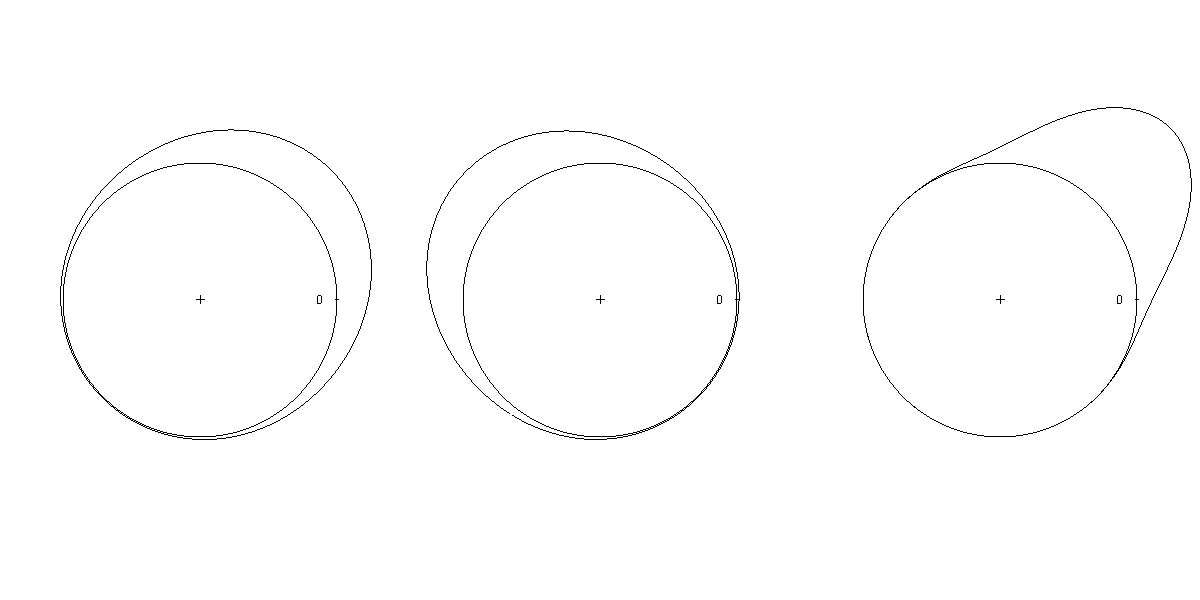
\includegraphics[width = 0.9\textwidth]{PN.pdf}
\caption{Projected normal densities with different $\boldsymbol{\mu}$. From left to right, the mean vector $\boldsymbol{\mu}$ is set to (2,2), (-2,2) and (4,4).} 
\label{figPN}
\end{figure}

In a circular regression model $\boldsymbol{\mu}$ may have the following
structure:

\begin{equation}\label{regression}
\boldsymbol{\mu}_{i} = \begin{pmatrix}
  \mu_{i}^{I}  \vspace{0.2cm}  \\
\mu_{i}^{II}
 \end{pmatrix}=\begin{pmatrix}
  (\boldsymbol{\beta}^{I})^{t}\boldsymbol{x}_{i}^{I} \vspace{0.2cm}  \\
  (\boldsymbol{\beta}^{II})^{t}\boldsymbol{x}_{i}^{II} 
 \end{pmatrix},
\end{equation}

where $i = 1, \dots, n$, $\boldsymbol{x}_{i}$ is a vector of predictor values
for individual $i$ and each $\boldsymbol{\beta}$ is a vector with intercept and
regression coefficients. To be able to estimate an intercept, the first
component of $\boldsymbol{x}_{i}$ equals 1. In this paper we center the
predictor $x$ and estimate the PN regression model using MCMC methods also used
in \cite{CremersMulderKlugkist2017}. Because the structure in (\ref{regression}) is
such that the predictor variables determine $\boldsymbol{\mu}$ the predictors
can have effects on both the mean (a location effect) and the variance (an
accuracy effect) of the circular outcome.





\section{Two indicators for accuracy and location effects}\label{indicators}

In this section we will describe two different indicators that allow us to check
whether the predictors in a projected normal regression model only have an
effect on the variance (an accuracy effect) or also have an effect on the
location (a location effect) of the circular outcome. The first indicator, the
$SSDO$, has been introduced previously in \cite{CremersMulderKlugkist2017}. The second
indicator is new and actually comprises a set of indicators that we call angle
based measures.

\subsection{The signed shortest distance to the origin ($SSDO$)}\label{measure1}

In \cite{CremersMulderKlugkist2017} it is outlined that the effects of a variable $x$
on both the variance and mean of the circular outcome in a PN regression model
can be detected by looking at the shortest distance of the regression line in
bivariate space to the origin ($SDO$). The regression line in $\mathbb{R}^2$ is
defined as follows: $$(\beta_0^I + \beta_1^Ix, \:  \beta_0^{II} +
\beta_1^{II}x)^t.$$

Figure \ref{figLocAcc} shows two regression lines in $\mathbb{R}^2$ together
with arrows representing predicted outcomes for $x = (x_{min}, 0, x_{max})$ and
a dotted line that represents the $SDO$. The intersections of the arrows with
the circle represent the predicted outcomes on the circle. The left figure shows
a situation with only an accuracy effect. In this situation the regression line
runs through the origin ($SDO = 0$) and the arrows for the predicted outcomes on
the circle are parallel and they intersect with the circle at one point, i.e.:
the circular predicted values for different values of $x$ are the same. The
right figure shows a situation where there is also a location effect. In this
situation the regression line does not run through the origin, $SDO > 0$ and the
arrows representing the predicted outcomes on the circle are not parallel and do
not intersect the circle at the same point, i.e.: the circular predicted values
for different values of $x$ are different.

The authors in \cite{CremersMulderKlugkist2017} introduced a measure, the signed shortest distance to
the origin ($SSDO$), derived from the $SDO$, to detect accuracy and location
effects. Just as for the $SDO$, \textit{$H_0: \text{There is only an
accuracy effect}$} is true for the $SSDO$ when it equals 0. To test whether
there is also a location effect with the $SSDO$ we can thus reformulate this
null hypothesis as \textit{$H_0: SSDO = 0$}. The authors in
\cite{CremersMulderKlugkist2017} make use of the highest posterior density (HPD) to
test the null hypothesis. The null hypothesis is rejected at a significance
level of $\alpha$ if the $100*(1-\alpha)$ HPD interval
for SSDO does not include zero.

The authors in \cite{CremersMulderKlugkist2017} perform a simulation for the $SSDO$. This simulation
  is however limited to two sample sizes and does not adequately investigate the
  validity of the test. With validity we mean achieving a correct type-I error
  in the long run. We will therefore  perform a new simulation with more sample
  sizes in Section \ref{simulation}. Additionally, we will set up this
  simulation such that it contains a larger variation of real $SDO$ values than
  before. Finally, we also include the new angle based measures (introduced
  next) in this simulation. This new set-up will allow us to assess and compare
  the type-I errors of the different measures.

\begin{figure}
\centering
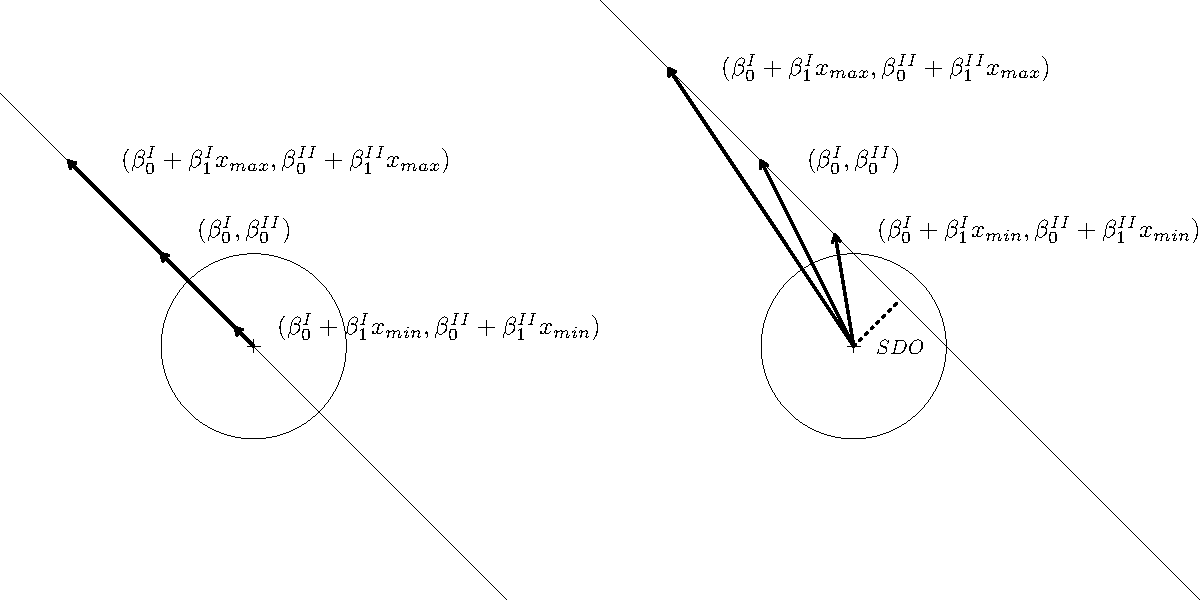
\includegraphics[width = 0.9\textwidth]{LocAcc.pdf}
\caption{Two regression lines in $\mathbb{R}^2$ together with a unit circle and arrows representing predicted outcomes for $x = (x_{min}, 0, x_{max})$ and the $SDO$.} 
\label{figLocAcc}
\end{figure}


\subsection{Angle based measures}\label{measure2}

In Figure \ref{figLocAcc} we saw that if the vectors representing predicted
values for several $x$ are not parallel there is a location effect. The new
measures we introduce in this section are based on testing whether these vectors
are parallel. A way to test whether two vectors are parallel is to compute the
sine of the angle between the two vectors and check whether this is equal to 0.
The sine of the angles $\lambda$ and $\gamma$ between the vectors $(\beta^I_0,
\beta^{II}_0)$ and $(\beta^I_0 + \beta^I_1x_{min}, \beta^I_0 +
\beta^{II}_1x_{min})$ and $(\beta^I_0 + \beta^I_1x_{max}, \beta^I_0 +
\beta^{II}_1x_{max})$ respectively from Figure \ref{figLocAcc} are computed as
follows:

\begin{equation}
\sin(\lambda) = \frac{\beta^I_0(\beta^{II}_0 + \beta^{II}_1x_{min}) - \beta^{II}_0(\beta^I_0 + \beta^{I}_1x_{min})}{\sqrt{(\beta^I_0)^2 + (\beta^{II}_0)^2}\sqrt{(\beta^{I}_0 + \beta^{I}_1x_{min})^2 + (\beta^{II}_0 + \beta^{II}_1x_{min})^2}}
\end{equation}

\begin{equation}
\sin(\gamma) = \frac{\beta^I_0(\beta^{II}_0 + \beta^{II}_1x_{max}) - \beta^{II}_0(\beta^I_0 + \beta^{I}_1x_{max})}{\sqrt{(\beta^I_0)^2 + (\beta^{II}_0)^2}\sqrt{(\beta^{I}_0 + \beta^{I}_1x_{max})^2 + (\beta^{II}_0 + \beta^{II}_1x_{max})^2}}
\end{equation}

\noindent and are bounded between -1 and 1. From now on we will call these measures
$\sin(\lambda)$ and $\sin(\gamma)$. Note that in this paper, because the
predictor $x$ has been centered, the vector $(\beta^I_0, \beta^{II}_0)$ is the
vector pointing at the data mean. We can thus reformulate \textit{$H_0:
\text{There is only an accuracy effect}$} as \textit{$H_0: \sin(\lambda) = 0$}
or \textit{$H_0: \sin(\gamma) = 0$}. We can test this null hypothesis by using
the 95$\%$ HPD interval of the posterior distribution of $\sin(\lambda)$ or
$\sin(\gamma)$. We could also measure the angle between the vectors for the
predicted values at $x_{min}$ and $x_{max}$. A reason to compute this other
measure is that the angle is always larger than either $\lambda$ or $\gamma$
on its own, which means that it may also have larger power for rejecting
\textit{$H_0$}. We define this measure as follows:

\begin{equation}
\sin(\lambda + \gamma) = \frac{(\beta^I_0 + \beta^{I}_1x_{min})(\beta^{II}_0 + \beta^{II}_1x_{max}) - (\beta^{II}_0 + \beta^{II}_1x_{min})(\beta^I_0 + \beta^{I}_1x_{max})}{\sqrt{(\beta^I_0 + \beta^{I}_1x_{min})^2 + (\beta^{II}_0 + \beta^{II}_1x_{min})^2}\sqrt{(\beta^{I}_0 + \beta^{I}_1x_{max})^2 + (\beta^{II}_0 + \beta^{II}_1x_{max})^2}}
\end{equation}

The three measures we have just introduced, $\sin(\lambda)$, $\sin(\gamma)$ and
$\sin(\lambda + \gamma)$, are all dependent on the shape of the data. For
testing purposes we would rather consider a measure that is not dependent on the
shape of the data. An intuitive way to construct such a measure is to consider
the vector $(\beta^I_1, \beta^{II}_1)$ and test whether this is parallel to
$(\beta^I_0, \beta^{II}_0)$:

\begin{equation}
\sin{\beta} = \frac{\beta^I_0\beta^{II}_1 - \beta^{II}_0\beta^{I}_1}{\sqrt{(\beta^I_0)^2 + (\beta^{II}_0)^2}\sqrt{(\beta^I_1)^2 + (\beta^{II}_1)^2}}.
\end{equation}

\noindent From now on we will call this measure $\sin(\beta)$. A visual representation of
$\beta$ is given in the left plot in Figure \ref{figDet}. The right plot shows
how $(\beta^I_1, \beta^{II}_1)$ is related to the regression line in bivariate
space; the addition of $(\beta^I_1, \beta^{II}_1)$ to $(\beta^I_0,
\beta^{II}_0)$ results in the vector $(\beta^I_0 + \beta^I_1, \beta^I_0 +
\beta^{II}_1)$.

Note that for all measures introduced above we could also use the cosine
formula, $\cos(\theta) = \boldsymbol{a} \boldsymbol{\cdot} \boldsymbol{b} /
||\boldsymbol{a}||||\boldsymbol{b}||)$, to compute the angle between two vectors
$\boldsymbol{a}$ and $\boldsymbol{b}$. However, the cosine of the angle between two vectors is -1 or 1 if they
are parallel, which is not convenient for the purpose of testing purposes.

\begin{figure}
\centering
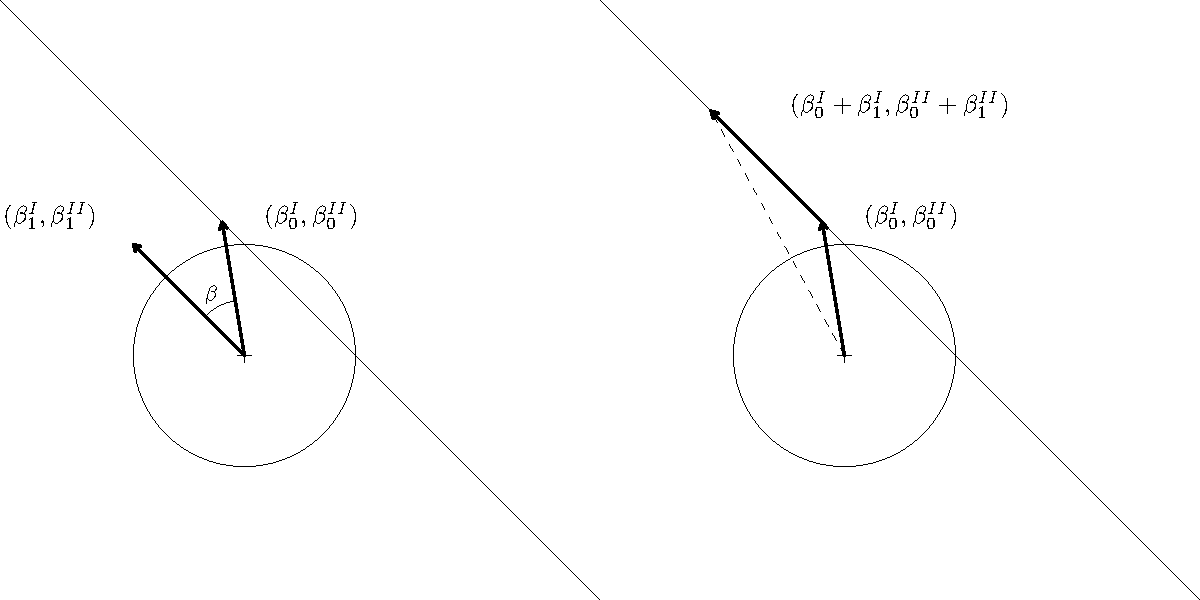
\includegraphics[width = 0.9\textwidth]{Determinant.pdf}
\caption{Visual representation of $\sin(\beta)$.} 
\label{figDet}
\end{figure}

\section{Simulation Study}\label{simulation}

To assess the performance of $SSDO$ and the angle based measures $\sin(\beta)$,
$\sin(\gamma)$, $\sin(\lambda)$ and $\sin(\lambda + \gamma)$ we conducted a
simulation study with 477 designs. In 72 of these designs,
the accuracy designs, there was only an accuracy effect ($SDO = 0$). In the
other designs, the location designs, there was also a location effect $SDO > 0$.

For each design 2500 datasets were simulated. These datasets had different
sample sizes ($N$): 25, 50, 75, 100 and 150. These sample sizes were chosen
because in earlier simulations for the $SSDO$ in \cite{CremersMulderKlugkist2017} only two
sizes (50 and 200) were used and in this paper we want to see more detailed
results regarding sample size. For each sample size 500 datasets were simulated.
Each dataset contains one circular outcome $\theta$ and one linear predictor $x
\sim N(0,1)$ similar to the simulation in \cite{CremersMulderKlugkist2017}. The relation
between predictor and outcome was determined by the population values for the
intercepts, $\beta_{0}^{I}$ and $\beta_{0}^{II}$, and coefficients,
$\beta_{1}^{I}$ and $\beta_{1}^{II}$. In each design different population values
were chosen for the intercepts and regression coefficients. For the designs with
a location effect pairs of population values $(\beta_{0}^{I},\beta_{0}^{II})$
for the linear intercepts were:

$$\{(\cos(10^\circ), \sin(10^\circ)), (\cos(30^\circ), \sin(30^\circ)), (\cos(45^\circ), \sin(45^\circ)), (\cos(60^\circ), \sin(60^\circ)), (\cos(80^\circ), \sin(80^\circ))\}$$
and pairs of population values for the regression coefficients $(\beta_{1}^{I},\beta_{1}^{II})$ were:

$$\{(1,0), (0,1) (1,1), (0.5,0), (0, 0.5), (0.5, 0.5), (2,0), (0,2), (2,2) \}.$$

\noindent These population values were then multiplied by a multiplication factor between
1 and 5 at intervals of 0.5 to obtain regression lines with different $SDO$.
Note that the coefficients were chosen to be largely similar to the coefficients
that show good performance (in terms of bias and coverage) in previous
simulation studies in \cite{CremersMulderKlugkist2017} and \cite{Cremers2018Assessing}.
Datasets for each possible combination of the pairs of intercepts and
regression coefficients and multiplication factors were simulated. These
combinations led to a larger variation in real $SDO$ values than in previous
simulations. In the accuracy designs the population values for $\beta_{0}^{I}$
and $\beta_{1}^{I}$ and $\beta_{0}^{II}$ and $\beta_{1}^{II}$ were equal in each
design. Their exact values and the simulation code is given in the supplementary
material.

From the population values of the intercepts and coefficients, the population
values of the $SDO$, $SSDO$ and the angle based measures ($\sin(\beta)$,
$\sin(\lambda)$ and $\sin(\gamma)$) were computed. For each dataset we determine
whether $x$ is predicted to have an accuracy effect by checking whether the
95$\%$ HPD intervals of the estimated $SSDO$ and the angle based measures
included 0. We thus test \textit{$H_0: \text{There is only an accuracy effect}$}. If
\textit{$H_0$} was not rejected the dataset was classified as having only an accuracy
effect. For each design we then computed the proportion of datasets in which the
$SSDO$ and the angle based measures indicated only an accuracy effect.

To display the results of the simulation in a concise manner, we grouped all
simulation designs into 6 categories based on their population $SDO$: those
where $SDO = 0$ (the 72 accuracy designs) and those where the $0 < SDO < 1$ (72
designs), $1 \leq SDO < 2$ (90 designs), $2 \leq SDO < 3$ (90 designs), $3 \leq
SDO < 4$ (90 designs) and $4 \leq SDO$ (63 designs). For each of the 6
categories of our simulation we then averaged the proportion of datasets where
only an accuracy effect was indicated over the designs of that category. For the
location designs this proportion represents a type-II error; the proportion in
which \textit{$H_0: \text{There is only an accuracy effect.}$} was not rejected even
though it should have been. For the accuracy designs this proportion is equal to
1 minus the type-I error of the test or actually the proportion in which we
correctly classify the effect as having only an accuracy effect. It also
represents the coverage of the HPD interval; we are testing whether the interval
includes 0 which is the real value in the accuracy designs. Thus, if the $SSDO$
and angle based measures perform well we expect the proportion to be high,
around 0.95 because we set $\alpha = 0.05$, for the accuracy designs and low for
the designs with a location effect. 


\subsection{Results}\label{results}

The results of the simulation are shown in Tables \ref{TableResSSDO} and
\ref{TableResdet} for the performance of the $SSDO$ and $\sin(\beta)$
respectively. The tables show the proportion of datasets in which \textit{$H_0:
\text{There is only an accuracy effect}$} could not be rejected grouped per real
$SDO$ value.

We see that for the location designs ($SDO > 0$) both measures perform better
with increasing sample sizes and with increasing $SDO$. The proportion of
datasets in which \textit{$H_0$} is not rejected ($SSDO$ = 0 or $\sin(\beta) =
0$) becomes lower when sample size and $SDO$ increase. For the accuracy designs
there is no clear effect of sample size for the $SSDO$. The proportion of
datasets in which \textit{$H_0$} is not rejected stays the same at around 0.9.
It thus does not reach the correct type-I error level (of 0.05) within the
current range of sample sizes. The fact that the actual alpha level consistently
seems to lie at 0.1 is not promising of the tests ability to reach the correct
alpha level asymptotically. There is an effect of sample size for $\sin(\beta)$
in the accuracy designs. This indicator reaches the correct type-I error level
at a sample size of 75 meaning that in the long run this is a valid test for
\textit{$H_0$}.

\begin{table}
\centering
\caption{The proportion of datasets in which an accuracy effect is indicated by $SSDO$ grouped per real $SDO$ value.} 
\begin{tabular}{lcccccc}
  \noalign{\smallskip}\hline\noalign{\smallskip}
$N$ & $SDO = 0$ & $ 0 < SDO < 1$ & $1 \leq SDO < 2$ & $2 \leq SDO < 3$ &  $3 \leq SDO < 4$ & $4 \leq SDO$\\ \hline\noalign{\smallskip}
25 & 0.90 & 0.49 & 0.23 & 0.14 & 0.10 & 0.06\\
50 & 0.89 & 0.35 & 0.15 & 0.10 & 0.08 & 0.05\\
75 & 0.90 & 0.28 & 0.12 & 0.08 & 0.07 & 0.05\\
100& 0.90 & 0.25 & 0.10 & 0.07 & 0.06 & 0.04\\
150& 0.89 & 0.19 & 0.08 & 0.06 & 0.06 & 0.04\\
   \hline
\end{tabular}
\label{TableResSSDO}
\end{table}

\begin{table}
\centering
\caption{The proportion of datasets in which an accuracy effect is indicated by $\sin(\beta)$ grouped per real $SDO$ value.} 
\begin{tabular}{lcccccc}
  \noalign{\smallskip}\hline\noalign{\smallskip}
$N$ & $SDO = 0$ & $ 0 < SDO < 1$ & $1 \leq SDO < 2$ & $2 \leq SDO < 3$ &  $3 \leq SDO < 4$ & $4 \leq SDO$\\ \hline\noalign{\smallskip}
25 & 0.91 & 0.52 & 0.27 & 0.17 & 0.13 & 0.08\\
50 & 0.92 & 0.39 & 0.18 & 0.12 & 0.09 & 0.06\\
75 & 0.94 & 0.33 & 0.14 & 0.09 & 0.07 & 0.05\\
100& 0.95 & 0.29 & 0.12 & 0.08 & 0.07 & 0.05\\
150& 0.94 & 0.23 & 0.10 & 0.07 & 0.06 & 0.04\\
   \hline
\end{tabular}
\label{TableResdet}
\end{table}

Results for the other three angle based measures, $\sin(\gamma)$,
$\sin(\lambda)$ and $\sin(\lambda + \gamma)$, are shown in the Appendix. In
general these measures perform worse or equal to $\sin(\beta)$. Only the
performance of $\sin(\gamma)$ stands out. This measure already reaches the
correct type-I error level for a sample size of 25. 





\section{Discussion}

In this paper we have introduced new angle based measures that allow testing of
\textit{$H_0: \text{There is only an accuracy effect}$} in projected normal regression
models for a circular outcome. We have investigated their performance and
compared these measures to a previously introduced measure, the $SSDO$ in a
simulation study.

The results of the simulation study lead us to conclude that in general the
angle based measures perform better than the $SSDO$ since three of them reach
the correct type-I error level in the long run. However, three of the four new
measures that we introduced in this paper, $\sin(\gamma)$, $\sin(\lambda)$ and
$\sin(\lambda + \gamma)$, are dependent on the distribution of the predictor
variable. In further research we could focus on finding more angle based
measures that are not dependent on the distribution of the predictor variable.
To do so standardization of the predictor $x$ instead of centering only could be
an option. Additionally now that we have found tests that have valid type-I
errors in the long run we can try to increase the power of these tests.

Lastly, we would like to note that in this paper we have only considered
simulation designs in which there is an effect in the population, either only an
accuracy effect or both an accuracy and a location effect. In reality however
there are situations in which there is no effect at all. In further research it
would be beneficial to investigate the performance of the $SSDO$ and the new
measures introduced here in samples for which there is no effect in the
population.

\section*{Acknowledgements}
We thank Irene Klugkist for insightful remarks and comments on the present
paper. Jolien Cremers acknowledges financial support from a Vidi grant awarded
to I. Klugkist from the Dutch Organization for Scientific Research (NWO
452‐12‐010).


\section{References}

\bibliographystyle{tfnlm}
\bibliography{CircularData.bib}




\section{Appendices}

\appendix

\begin{table}[ht]
\centering
\caption{The proportion of datasets in which an accuracy effect is indicated by $\sin(\lambda)$ grouped per real $SDO$ value.} 
\begin{tabular}{lcccccc}
  \noalign{\smallskip}\hline\noalign{\smallskip}
$N$ & $SDO = 0$ & $ 0 < SDO < 1$ & $1 \leq SDO < 2$ & $2 \leq SDO < 3$ &  $3 \leq SDO < 4$ & $4 \leq SDO$\\ \hline\noalign{\smallskip}
25 & 0.90 & 0.50 & 0.25 & 0.16 & 0.12 & 0.07\\
50 & 0.89 & 0.38 & 0.16 & 0.11 & 0.08 & 0.05\\
75 & 0.92 & 0.31 & 0.13 & 0.09 & 0.07 & 0.05\\
100& 0.93 & 0.27 & 0.11 & 0.08 & 0.07 & 0.05\\
150& 0.93 & 0.22 & 0.09 & 0.07 & 0.06 & 0.04\\
   \hline
\end{tabular}
\label{TableResdetmin}
\end{table}

\begin{table}[ht]
\centering
\caption{The proportion of datasets in which an accuracy effect is indicated by $\sin(\gamma)$ grouped per real $SDO$ value.} 
\begin{tabular}{lcccccc}
  \noalign{\smallskip}\hline\noalign{\smallskip}
$N$ & $SDO = 0$ & $ 0 < SDO < 1$ & $1 \leq SDO < 2$ & $2 \leq SDO < 3$ &  $3 \leq SDO < 4$ & $4 \leq SDO$\\ \hline\noalign{\smallskip}
25 & 0.94 & 0.56 & 0.28 & 0.18 & 0.13 & 0.08 \\
50 & 0.94 & 0.42 & 0.18 & 0.12 & 0.09 & 0.05 \\
75 & 0.95 & 0.34 & 0.14 & 0.09 & 0.07 & 0.05 \\
100& 0.95 & 0.30 & 0.12 & 0.08 & 0.07 & 0.05 \\
150& 0.95 & 0.23 & 0.10 & 0.07 & 0.06 & 0.04 \\
   \hline
\end{tabular}
\label{TableResdetmax}
\end{table}

\begin{table}[ht]
\centering
\caption{The proportion of datasets in which an accuracy effect is indicated by $\sin(\gamma+ \lambda)$ grouped per real $SDO$ value.} 
\begin{tabular}{lcccccc}
  \noalign{\smallskip}\hline\noalign{\smallskip}
$N$ & $SDO = 0$ & $ 0 < SDO < 1$ & $1 \leq SDO < 2$ & $2 \leq SDO < 3$ &  $3 \leq SDO < 4$ & $4 \leq SDO$\\ \hline\noalign{\smallskip}
25 & 0.91 & 0.53 & 0.25 & 0.16 & 0.12 & 0.07 \\
50 & 0.92 & 0.39 & 0.17 & 0.11 & 0.08 & 0.05 \\
75 & 0.94 & 0.32 & 0.13 & 0.09 & 0.07 & 0.05 \\
100& 0.95 & 0.28 & 0.11 & 0.08 & 0.07 & 0.05 \\
150& 0.95 & 0.23 & 0.09 & 0.07 & 0.06 & 0.04 \\
   \hline
\end{tabular}
\label{TableResdetminmax}
\end{table}

\end{document}
